\chapter{Structure de la base de données}

\section{Structure générale du schéma otolithe}
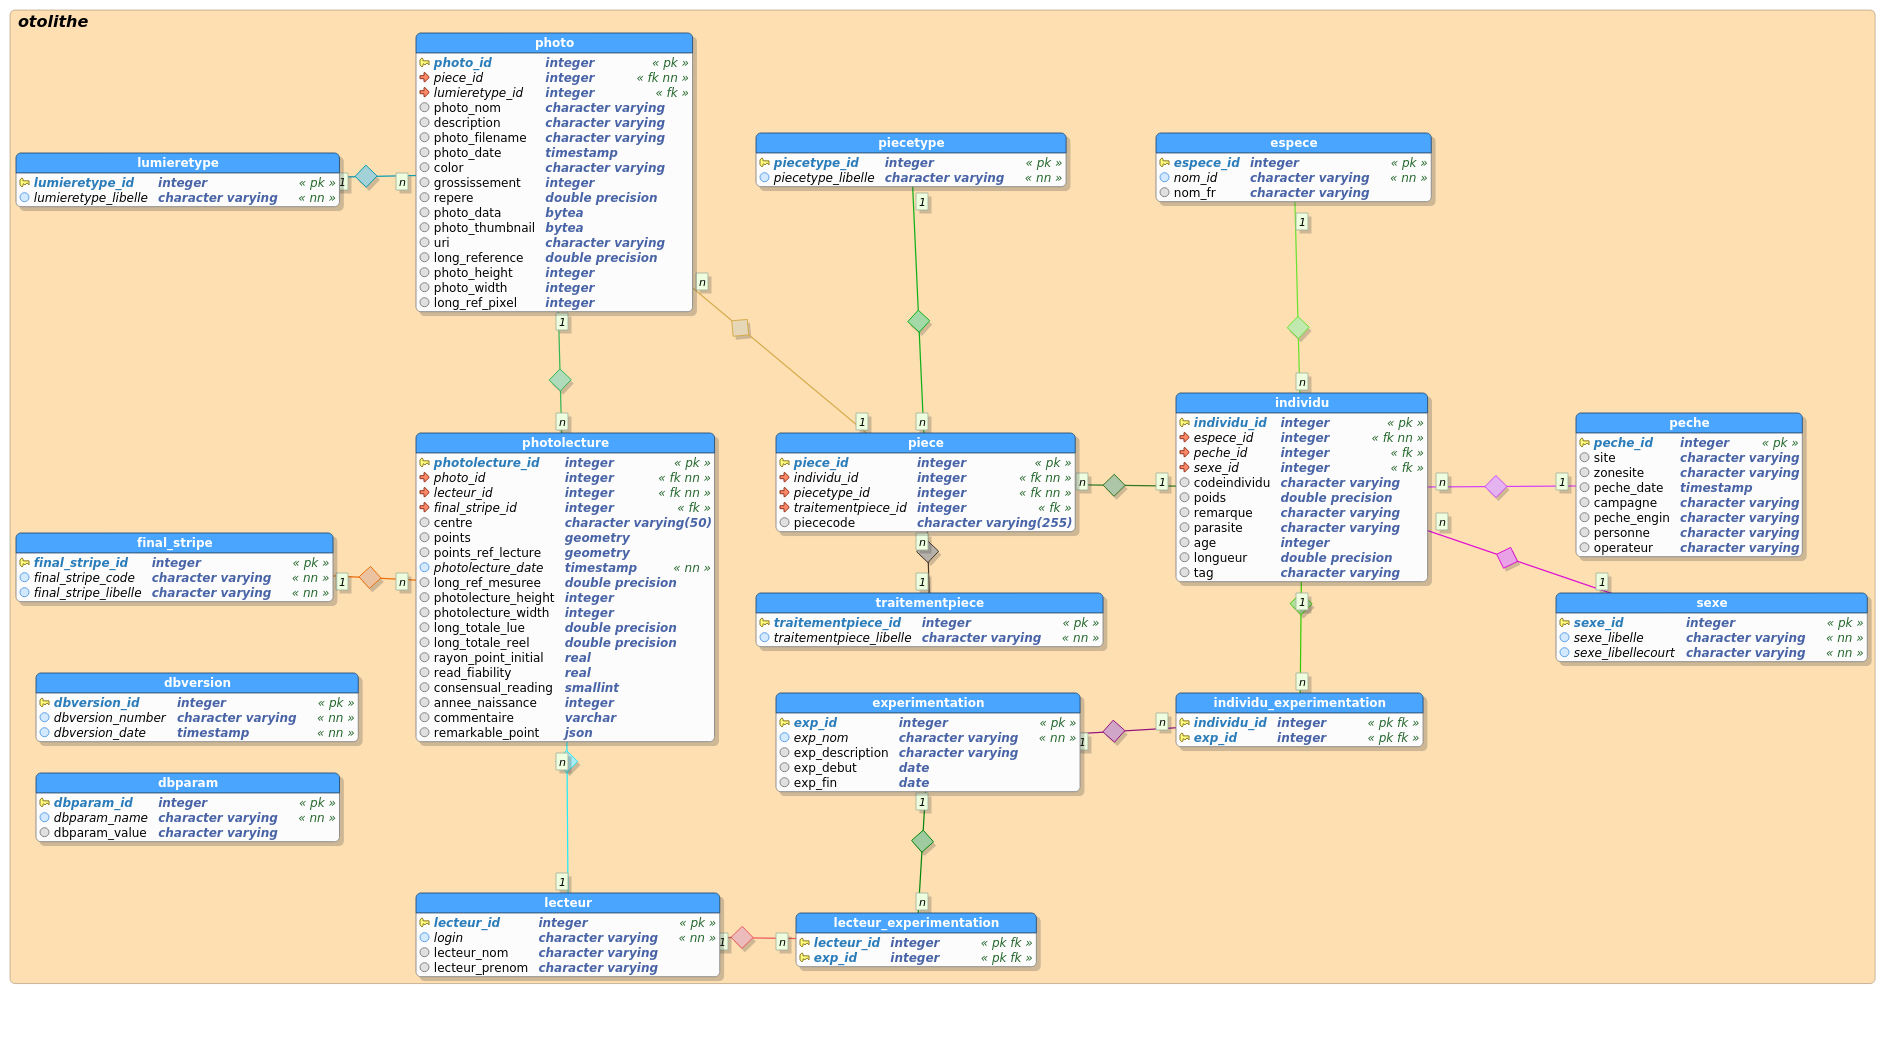
\includegraphics[width=\linewidth
%,angle=90
]{otolithe.png}

\section{Description des tables du schéma otolithe}
\subsection{dbparam}
Table des parametres associes de maniere intrinseque a l'instance

\begin{tabular}{|l| p{2cm}|c|c|c| p{3cm}|}
\hline
Column name & Type & Not null & Key & Foreign key & Comment \\
\hline
dbparam\_id & integer & X & X & & \\
\hline
dbparam\_name & character varying & X & & & Nom du parametre\\
\hline
dbparam\_value & character varying & & & & Valeur du paramètre\\
\hline
\end{tabular}
\subsection{dbversion}
Table des versions de la base de donnees

\begin{tabular}{|l| p{2cm}|c|c|c| p{3cm}|}
\hline
Column name & Type & Not null & Key & Foreign key & Comment \\
\hline
dbversion\_id & integer & X & X & & \\
\hline
dbversion\_number & character varying & X & & & Numero de la version\\
\hline
dbversion\_date & timestamp without time zone & X & & & Date de la version\\
\hline
\end{tabular}
\subsection{espece}
Liste des especes

\begin{tabular}{|l| p{2cm}|c|c|c| p{3cm}|}
\hline
Column name & Type & Not null & Key & Foreign key & Comment \\
\hline
espece\_id & integer & X & X & & \\
\hline
nom\_id & character varying & X & & & \\
\hline
nom\_fr & character varying & & & & \\
\hline
\end{tabular}
\subsection{experimentation}
Experimentation a laquelle est rattache le poisson

\begin{tabular}{|l| p{2cm}|c|c|c| p{3cm}|}
\hline
Column name & Type & Not null & Key & Foreign key & Comment \\
\hline
exp\_id & integer & X & X & & \\
\hline
exp\_nom & character varying & X & & & \\
\hline
exp\_description & character varying & & & & \\
\hline
exp\_debut & date & & & & \\
\hline
exp\_fin & date & & & & \\
\hline
\end{tabular}
\subsection{final\_stripe}
Natures de la strie finale

\begin{tabular}{|l| p{2cm}|c|c|c| p{3cm}|}
\hline
Column name & Type & Not null & Key & Foreign key & Comment \\
\hline
final\_stripe\_id & integer & X & X & & \\
\hline
final\_stripe\_code & character varying & X & & & Code utilisé\\
\hline
final\_stripe\_libelle & character varying & X & & & \\
\hline
\end{tabular}
\subsection{lecteur}
personne realisant la lecture d'une photo

\begin{tabular}{|l| p{2cm}|c|c|c| p{3cm}|}
\hline
Column name & Type & Not null & Key & Foreign key & Comment \\
\hline
lecteur\_id & integer & X & X & & \\
\hline
login & character varying & X & & & \\
\hline
lecteur\_nom & character varying & & & & \\
\hline
lecteur\_prenom & character varying & & & & \\
\hline
\end{tabular}
\subsection{lecteur\_experimentation}
Table des experimentations autorisees pour un lecteur

\begin{tabular}{|l| p{2cm}|c|c|c| p{3cm}|}
\hline
Column name & Type & Not null & Key & Foreign key & Comment \\
\hline
lecteur\_id & integer & X & X & X & \\
\hline
exp\_id & integer & X & X & X & \\
\hline
\end{tabular}
\subsection{peche}
Date de peche et lieu de capture

\begin{tabular}{|l| p{2cm}|c|c|c| p{3cm}|}
\hline
Column name & Type & Not null & Key & Foreign key & Comment \\
\hline
peche\_id & integer & X & X & & \\
\hline
site & character varying & & & & \\
\hline
zonesite & character varying & & & & \\
\hline
peche\_date & timestamp without time zone & & & & \\
\hline
campagne & character varying & & & & \\
\hline
peche\_engin & character varying & & & & \\
\hline
personne & character varying & & & & \\
\hline
operateur & character varying & & & & \\
\hline
\end{tabular}
\subsection{photo}
photos associees a une piece

\begin{tabular}{|l| p{2cm}|c|c|c| p{3cm}|}
\hline
Column name & Type & Not null & Key & Foreign key & Comment \\
\hline
photo\_id & integer & X & X & & \\
\hline
piece\_id & integer & X & & X & \\
\hline
lumieretype\_id & integer & & & X & \\
\hline
photo\_nom & character varying & & & & \\
\hline
description & character varying & & & & \\
\hline
photo\_filename & character varying & & & & \\
\hline
photo\_date & timestamp without time zone & & & & \\
\hline
color & character varying & & & & \\
\hline
grossissement & integer & & & & \\
\hline
repere & double precision & & & & \\
\hline
photo\_data & bytea & & & & \\
\hline
photo\_thumbnail & bytea & & & & \\
\hline
uri & character varying & & & & \\
\hline
long\_reference & double precision & & & & \\
\hline
photo\_height & integer & & & & Hauteur de la photo originale\\
\hline
photo\_width & integer & & & & Largeur de la photo originale\\
\hline
long\_ref\_pixel & integer & & & & Longueur de reference en pixels - valeur par defaut pour photolecture, si non lu\\
\hline
\end{tabular}
\subsection{photolecture}
Lecture realisee par une personne

\begin{tabular}{|l| p{2cm}|c|c|c| p{3cm}|}
\hline
Column name & Type & Not null & Key & Foreign key & Comment \\
\hline
photolecture\_id & integer & X & X & & \\
\hline
photo\_id & integer & X & & X & \\
\hline
lecteur\_id & integer & X & & X & \\
\hline
final\_stripe\_id & integer & & & X & \\
\hline
centre & character varying & & & & \\
\hline
points & geometry & & & & \\
\hline
points\_ref\_lecture & geometry & & & & Emplacement des points utilises pour lire la longueur de reference\\
\hline
photolecture\_date & timestamp without time zone & X & & & \\
\hline
long\_ref\_mesuree & double precision & & & & \\
\hline
photolecture\_height & integer & & & & Hauteur de la photo utilisee pour la lecture\\
\hline
photolecture\_width & integer & & & & Largeur de la photo affichee pour realiser la lecture\\
\hline
long\_totale\_lue & double precision & & & & Somme des segments entre chacun des points\\
\hline
long\_totale\_reel & double precision & & & & Longueur totale réelle calculée pour le lecteur (long\_reference / long\_ref\_mesuree * long\_totale\_lue)\\
\hline
rayon\_point\_initial & real & & & & \\
\hline
read\_fiability & real & & & & Fiabilité de la lecture\\
\hline
consensual\_reading & smallint & & & & 1 si lecture consensuelle\\
\hline
annee\_naissance & integer & & & & Année de naissance estimée\\
\hline
commentaire & character varying & & & & Commentaires de lecture\\
\hline
remarkable\_points & json & & & & Liste des points remarquables identifiés sur la photo\\
\hline
\end{tabular}
\subsection{piece}
Pieces analysees

\begin{tabular}{|l| p{2cm}|c|c|c| p{3cm}|}
\hline
Column name & Type & Not null & Key & Foreign key & Comment \\
\hline
piece\_id & integer & X & X & & \\
\hline
individu\_id & integer & X & & X & \\
\hline
piecetype\_id & integer & X & & X & \\
\hline
traitementpiece\_id & integer & & & X & \\
\hline
piececode & character varying & & & & \\
\hline
\end{tabular}
\subsection{piecetype}
Type de piece

\begin{tabular}{|l| p{2cm}|c|c|c| p{3cm}|}
\hline
Column name & Type & Not null & Key & Foreign key & Comment \\
\hline
piecetype\_id & integer & X & X & & \\
\hline
piecetype\_libelle & character varying & X & & & \\
\hline
\end{tabular}